\chapter{Implementación JPEG}\label{ch:implementacion}

Este trabajo empezó como un proyecto motivado por curiosidad para averiguar
cómo funciona JPEG. La idea de usar el GPU salió de notar que el algoritmo
separa a la imagen en bloques que parecían ser independientes. En realidad no
lo son, pero como se verá mas adelante, se encontró una manera de hacer un
codificador paralelo. El progreso culminó en lo que se describe en este
trabajo. El proyecto final se le llamó \emph{gp\_encoder} y su código está en
github \cite{gp_encoder}.

El codificador JPEG fue lanzado al dominio público en \emph{ Github } bajo el
nombre de TinyJPEG \cite{tiny_jpeg}.

En este capítulo se describen los detalles de ambos proyectos.

\section {Términos}

Se usan los términos \emph{\gls{depurar}} y
\emph{\gls{profiling}}. Depurar, en computación, se refiere al proceso de
encontrar y arreglar defectos de código. \emph{profiling} es el proceso de
encontrar los puntos en los que un programa puede ser modificado para mejorar
el desempeño.

El término \emph{multihilo} se usa para referirse a la arquitectura CPU que
puede ejecutar múltiples hilos de ejecución en un mismo procesador.

\emph{General Purpose GPU}, o \emph{\gls{GPGPU}} es el término usado para la
práctica de programar GPU directamente, a diferencia del uso original, donde
el GPU era un acelerador controlado por una biblioteca de gráficas como OpenGL
o DirectX.

% ============================================================
\section{Tecnologías}
% ============================================================

La elección de lenguaje para TinyJPEG fue C. C99 para ser específico
\cite{c99}. TinyJPEG fue lanzado con el objetivo de ser una biblioteca
reutilizable, y ha encontrado cierto grado de éxito. Un planetario en París usa
TinyJPEG para capturar vídeo de sus simulaciones.

C es un lenguaje ideal para escribir cosas como codificadores. El lenguaje
permite mantener el nivel bajo de abstracción que se necesita y las
herramientas de \emph{debugging} son mejores para C y C++ que para casi
cualquier otro lenguaje.

Se escogió OpenCL para la implementación de GPGPU. OpenCL es un estándar abierto
para GPGPU y está soportado por Intel, Nvidia y AMD. La máquina en la que se
implementó este trabajo tiene una tarjeta Nvidia. Nvidia tiene su propio
lenguaje para GPGPU, llamado CUDA, que tiene mejor soporte para debugging y
profiling que OpenCL para sus tarjetas de video. Sin embargo, las herramientas
siguen siendo primitivas comparadas con lo que se tiene en el CPU. En cualquier
caso, uno termina haciendo hipótesis, experimentos y mediciones para optimizar la
solución, aun teniendo herramientas sofisticadas. Se escogió OpenCL porque los
méritos relativos de facilidad de desarrollo de CUDA no le ganan al soporte
multi-plataforma y al valor de apoyar estándares abiertos de OpenCL.


% ============================================================
\section{Arquitectura}
% ============================================================

TinyJPEG es minimalista. Consiste de un archivo de alrededor 1000 líneas. Está
escrito en el estilo popularizado por Sean Barrett \footnote{Sean Barrett es un
programador famoso por escribir el motor de rendering del juego Thief y de sus
bibliotecas de código libre \emph{stb} para facilitar el desarollo de
aplicaciones multimedia.} de escribir un solo archivo \verb+.h+ con la
siguiente estructura:

\label{alg:stb}
\begin{code}[language=C][h]
    // Principio del archivo
    #pragma once

    // Definición de la interfaz.
    tje_encode_to_file(...);

    #ifdef TJE_IMPLEMENTATION

    // La implementación completa va aquí.
\end{code}

De esta manera, uno puede incluir \verb+#include <tiny_jpeg.h>+ como cualquier
encabezado de C, pero en uno de los archivos del proyecto, para definir la
implementación completa, se hace lo siguiente.

\label{alg:stb_impl}
\begin{code}[language=C][h]
    #define TJE_IMPLEMENTATION
    #include <tiny_jpeg.h>
\end{code}

El propósito de esta técnica es facilitar la distribución de bibliotecas en un
lenguaje que no cuenta con un sistema de distribución digital, o siquiera un
sistema de módulos.

Se exponen dos funciones como interfaz pública:

\begin{code}[language=C][h]
tje_encode_to_file(...)
tje_encode_to_file_at_quality(...)
\end{code}

La primera comprime con la tabla unitaria y la segunda ofrece tres posibles
niveles de calidad: ``alto", ``mediano", y ``bajo". Todos correspondientes
únicamente al uso de tres tablas de cuantificación.

Ambas funciones son envolturas sobre la función principal interna, que funciona
de la siguiente manera:

Se prepara una estructura estática para hacer compresión de Huffman y se
pre-procesa la tabla según el algoritmo DCT descrito en \ref{sec:DCT}. A esto
le llamamos el \emph{paso inicial}.  Cuando terminamos el \emph{paso inicial},
determinamos el número de bloques que van a ser procesados. JPEG debe poder
funcionar con imágenes cuyos tamaños verticales y horizontales no sean múltiplos
de 8. Para esto la especificación sólo nos pide como codificador redondear al
siguiente múltiplo de 8. Al decodificador le pide ignorar los datos adicionales. Para
evitar \gls{artefactos}, como convención se repite en el bloque el color del
último píxel de la imagen para cada columna adicional y para cada renglón adicional. Si
$w$ es el ancho de la imagen y $h$ es el alto, y ninguno de los dos es múltiplo
de 8, entonces el número de bloques es $n = (w + (8 - w \mod 8)) * (h + (8 - h
\mod 8))$. Cuando $w$ o $h$ es múltiplo de ocho, entonces se sustituye el
término en la multiplicación por solamente $w$ o $h$ respectivamente. Por
ejemplo, si $w \mod 8 = 0$ entonces $n = w * (h + (8 - h \mod 8))$

Cada bloque se separa en tres bloques \verb+Y+, \verb+U+, \verb+V+, a los que
se les aplica la función \verb+encode_MCU()+.

La función \verb+encode_MCU()+ se llama así por el acrónimo \emph{\gls{MCU}},
\emph{Minimum Coded Unit}. JPEG puede especificar un factor para describir los
bloques \verb+U+ y \verb+V+ con menos resolución, por nuestra relativa falta de
sensibilidad a la crominancia contra la luminancia, pero TinyJPEG no utiliza
esto. Otra posibilidad es usar diferentes tablas de codificación para
lumninancia y crominancia. TinyJPEG sí utiliza esto, escogiendo tablas con
mayor compresión para los bloques de crominancia.

Se usa un par de iteraciones para extraer los bloques, y cada bloque se pasa como
parámetro a la función \verb+encode_MCU+. En pseudo-código:

\begin{code}[language=C][h]
    for ( int y = 0; y < height; y += 8 ) {
        for ( int x = 0; x < width; x += 8 ) {
            for ( int off_y = 0; off_y < 8; ++off_y ) {
                for ( int off_x = 0; off_x < 8; ++off_x ) {
                    int block_index = (off_y * 8 + off_x);
                    // ... llenar bloque
                }
            }
            encode_MCU(bloque);
        }
    }
\end{code}

\subsection{DummyJPEG} \label{sub:dummy}

A primera vista, el algoritmo JPEG se ve ``embarazosamente paralelo". Una
motivación para este trabajo fue la observación de que el algoritmo trabaja
dividiendo la imágenes en cuadros de $8\times8$ y el hecho de que los GPU
actuales trabajan con instrucciones vectoriales de 32 elementos. Actualmente,
cuando se hace \gls{GPGPU}, se considera buena práctica que el tamaño de las
unidades de trabajo sean un múltiplo de la longitud de las instrucciones de la
arquitectura. Por esto, los bloques de 64 elementos se prestan a ser procesados
por GPU actuales.

Desafortunadamente, el algoritmo JPEG no es paralelo. Aplicar codificación
delta al coeficiente DC introduce una dependencia de datos entre cada bloque de
\verb+Y+, \verb+U+ y \verb+V+ respectivamente. Para cada componente, cualquier
bloque después del primero depende del anterior para poder computar la
diferencia entre su coeficiente DC  y el de su antecesor.

Sin embargo, aunque JPEG es inherentemente secuencial para cada componente,
está muy cerca de ser paralelo. Si el \emph{Joint Photographic Experts Group}
no hubiera decidido tratar de manera diferente a los \gls{coeficientes AC} y DC, el
algoritmo sería completamente paralelo.

Se quiere darle la vuelta al problema, y la manera en que se hace es creando
un ``Dummy JPEG": Un algoritmo que es \emph{casi} JPEG, pero que no es correcto.

La implementación de DummyJPEG empieza como un clon directo de TinyJPEG. Lo
primero que se hace es cambiar las función que escribe a disco por una función
que va contando el número de bits. De esta manera, al aplicar el algoritmo no
se tiene una imagen, pero se tiene un reporte del tamaño de la imagen que
se hubiera generado.

También se cambia el algoritmo para aplicar la Transformada Inversa de Coseno
justo después de aplicar la DCT al bloque, para poder compararlos y calcular el
error.

Entonces, si el algoritmo original para cada bloque en TinyJPEG es:

\begin{code}
    x = aplicar_dct(bloque);
    codificar(x)
\end{code}

El algoritmo para cada bloque en DummyJPEG se convierte en esto:

\begin{code}
    x = aplicar_dct(bloque)
    reportar_tamaño(x)
    y = aplicar_idct(x)
    reportar_error(bloque, y)
\end{code}

En donde \verb+reportar_error+ es una suma de la diferencia absoluta entre cada
pixel del bloque original y del bloque reconstruido.

La manera en que se vuelve paralelo a DummyJPEG es simplemente no codificar al
coeficiente DC. Esto introduce un error en el tamaño reportado pero no afecta
al error reportado. El error que se introduce viene de que se cuentan los bits de
la representación de los 63 \gls{coeficientes AC}, pero no se cuentan los bits del
\gls{coeficiente DC}. En las imágenes de prueba que se usaron para este trabajo, el
tamaño reportado es menor que el tamaño real entre un 10\% y 20\%.

La pregunta que se hace es: ¿El error en el reporte de tamaño es significativo?

La presión que se pone en la evolución es hacia imágenes que son
indistinguibles de la original. Como el valor de cuantificación del primer
coeficiente afecta de manera importante la calidad de imagen comprimida, las
tablas de la población rápidamente convergen a tener el primer valor de
cuantificación igual a 1. Esto quiere decir que para casi cualquier conjunto de
tablas que vayamos a comparar, su coeficiente DC es igual. Por lo tanto,
siempre se introduce el mismo error en el reporte de los tamaños de las
imágenes resultantes. Esto nos permite despreocuparnos de no tomar en cuenta el
primer coeficiente.

Otra cosa que se hace es \emph{solo calcular bloques de luminancia}, ya que los
bloques de crominancia usualmente usan una tabla secundaria y el propósito es
evolucionar una sola tabla. Podemos deshacernos de $66\%$ del trabajo si
descartamos los dos componentes de crominancia. Más tarde, cuando se finalice
la evolución, podemos usar la misma tabla para los tres componentes o bajar la
calidad de la tabla para los componentes de crominancia, multiplicando cada
elemento por alguna constante.

Ya que se tiene un algoritmo que es \emph{casi JPEG}, pero paralelo, se sigue
con la tarea de cambiar la arquitectura del programa para paralelizarlo en el
CPU. La razón por la que se implementa el paralelismo en el CPU antes de
hacerlo en el GPU es principalmente la velocidad de desarrollo. La versión
paralela en el CPU se hace pensando en el diseño final para el GPU.  El
código se moldea para que el flujo de ejecución en el CPU sea muy similar a la
manera en que trabaja el GPU, intentando llegar al punto en que la
implementación en el GPU se reduzca a un \emph{copy paste}, pero que el esfuerzo
que se aplique a la implementación del GPU sea solamente un trabajo de
optimización de bajo nivel.

\section{Introducción a GPGPU} \label{sec:gpgpu}

Las arquitecturas de GPU, en el momento que se escribe esto, trabajan con
instrucciones SIMT (\emph{Single Instruction, Multiple Threads}).

Supercomputadoras vectoriales como la \emph{Cray} se introdujeron en la década
de 1970 pero gradualmente perdieron popularidad, mientras computadoras con
microprocesadores x86 bajaron de precio. Las computadoras de escritorio serían
completamente escalares hasta el final de los 90, y las súper-computadoras
seguirían siendo por un tiempo grupos de procesadores x86.

En 1998 AMD introdujo instrucciones vectoriales con su tecnología \emph{3D
Now}, seguido por Intel en 1999 cuando introdujo SSE (Streaming SIMD
extensions). Ambas tecnologías son extensiones al conjunto de instrucciones x86
que introducen cómputo vectorial. Unos años más tarde se empezarían a
popularizar los procesadores \emph{multi-core}. Ambos desarrollos, que
introducen cómputo paralelo a los procesadores para consumidor, son el resultado
de la desaceleración de la velocidad escalar y una demanda constante de mayor desempeño.

Otra respuesta a esta demanda para mayor desempeño nació en los noventas: Los
aceleradores gráficos o GPU, tarjetas que se dedican a rasterizar triángulos
rápidamente para aplicaciones multimedia, principalmente videojuegos.

Aunque al principio los GPU estaban diseñados alrededor de  las API como OpenGL y
DirectX, con funcionalidad fija, poco a poco fueron adquiriendo la habilidad de
ser programables. Primero con \emph{shaders}, que permitieron meter código en
un par de partes clave del proceso de rasterización, y más tarde con OpenCL y
CUDA, que permiten escribir programas para el GPU en un dialecto de C.

El modelo de ejecución de OpenCL corresponde directamente a las arquitecturas
GPU actuales. Para describir su funcionamiento, en este documento se usa la
terminología de OpenCL y AMD. Nvidia tiene términos diferentes para los mismos
conceptos, la tabla \ref{table:equiv} describe las equivalencias.

Esta descripción se enfoca en la arquitectura Kepler de Nvidia y cómo le
corresponden los conceptos de OpenCL.

Un programa OpenCL opera con \emph{work items}. Un \emph{work item} puede pensarse
como una \emph{``fibra"} en un \emph{``cable"} que ejecuta instrucciones
vectoriales. En la arquitectura moderna de Nvidia, la longitud de los
vectores es de 32 elementos. Es decir, cada cable tiene 32 fibras.

A estos \emph{``cables"} se les denomina \emph{wavefronts}.

La tarjeta de video tiene un calendarizador implementado en hardware que
trabaja con granularidad de \emph{wavefronts} individuales. Los \emph{work
items} corren \emph{kernels}, que son funciones escritas en el dialecto de C de
OpenCL para ser ejecutadas en el GPU. Un kernel de OpenCL se ve como código en
C, pero hay que imaginarse que en lugar de un sólo apuntador de instrucciones
avanzando secuencialmente, se está lidiando con 32 apuntadores de instrucciones
(las fibras del cable en la analogía que se usa). Este es un paradigma
diferente. Por ejemplo, los saltos dinámicos se convierten en algo caro, ya que
mientras un subconjunto de los 32 apuntadores de instrucciones procesa un
camino de ejecución, el resto debe esperar. Un salto que se toma el 50\% del
tiempo es causa una reducción de velocidad de 2x.

Un \emph{work item} es parte de un \emph{work item}. El tamaño del
\emph{work group} es decisión del programador, puede ser de 1, 2 o 3
dimensiones y su tamaño puede variar, aunque es buena práctica escoger un
múltiplo del tamaño de los wavefronts (32 en Kepler y Maxwell). Hay que
encontrar el tamaño apropiado para los \emph{work items} para minimizar
contención de memoria y maximizar el rendimiento (se usa la palabra rendimiento
como traducción directa de de \emph{throughput}). Los GPU están diseñados para
sacrificar latencia por rendimiento.

Nótese que el concepto de \emph{work item} es una abstracción que se
provee para facilitar la programación en OpenCL. Crear \emph{work items} de
cierto tamaño y dimensiones ayuda a visualizar problemas. Sin embargo, es
importante tener siempre en cuenta que un \emph{work item} siempre es ejecutado
por un \emph{wavefront}.

Cada generación de GPU tiene diferentes características de desempeño. Es útil
usar referencias oficiales \cite{maxwell-tuning}, pero los recursos gratis,
como GPU Tech Conf (GTC) \cite{gtc}, una conferencia anual sobre GPU, son una
buena fuente de información para aprender a obtener el mayor desempeño posible
de las arquitecturas actuales.

En la microarquitectura del GPU, los \emph{wavefronts} son ejecutados en
procesadores vectoriales llamados \emph{Processing Elements}. Cada \emph{ Processing
Element } tiene un número limitado de registros y puede ejecutar un \emph{wavefront} a la vez.

Cada \emph{ Processing Element } es miembro de un \emph{Compute Unit}, que tiene un caché L1.

El GPU contiene un número de \emph{ Compute Units }, quienes comparten un caché L2 y una
memoria global. En el ejemplo en la figura \ref{fig:kepler1} es un GPU con 15
\emph{ Compute Units }.

Desde el punto de vista del modelo OpenCL solo existe la memoria local y
memoria global. En la práctica, la memoria local corresponde a los registros
del \emph{ Processing Element } y al cache L1. La memoria global corresponde a la
memoria global del GPU, pero la microarquitectura puede encargarse de ``subir''
y ``bajar''  accesos de memoria global por la jerarquía de memoria física.

Durante la ejecución de un kernel. A diferencia de los CPU, no hay garantía de
coherencia cuando se escribe a memoria. OpenCL provee mecanismos de
sincronización de memoria para cuando es absolutamente necesario, pero en la
práctica resultan en un golpe fuerte al desempeño.

La arquitectura de los GPU está diseñada para lidiar con problemas de
contención de memoria. Cuando algún \emph{work item} dentro de un \emph{wavefront} está
esperando a que se efectúe una operación de memoria, o está esperando a otro
miembro del \emph{wavefront} a causa de un salto condicional, el calendarizador hace
que el \emph{compute unit} ejecute otro \emph{wavefront} que esté listo para ser
ejecutado. Esto ocurre muy rápidamente, no hay un costo alto de cambio de
contexto como al que estamos acostumbrados con hilos en sistemas operativos.

Las figuras \ref{fig:kepler1} y \ref{fig:kepler2}, tomadas de la plática de
Nvidia ``Inside Kepler" \cite{kepler-slides}, ayudan a visualizar cómo
corresponde el modelo OpenCL a una arquitectura GPU. En el caso de Kepler,
podemos ver un SMX como un \emph{ Compute Unit }, y cada \emph{ Cuda Core } como un \emph{ Processing Element }.

\begin{figure}[h]
    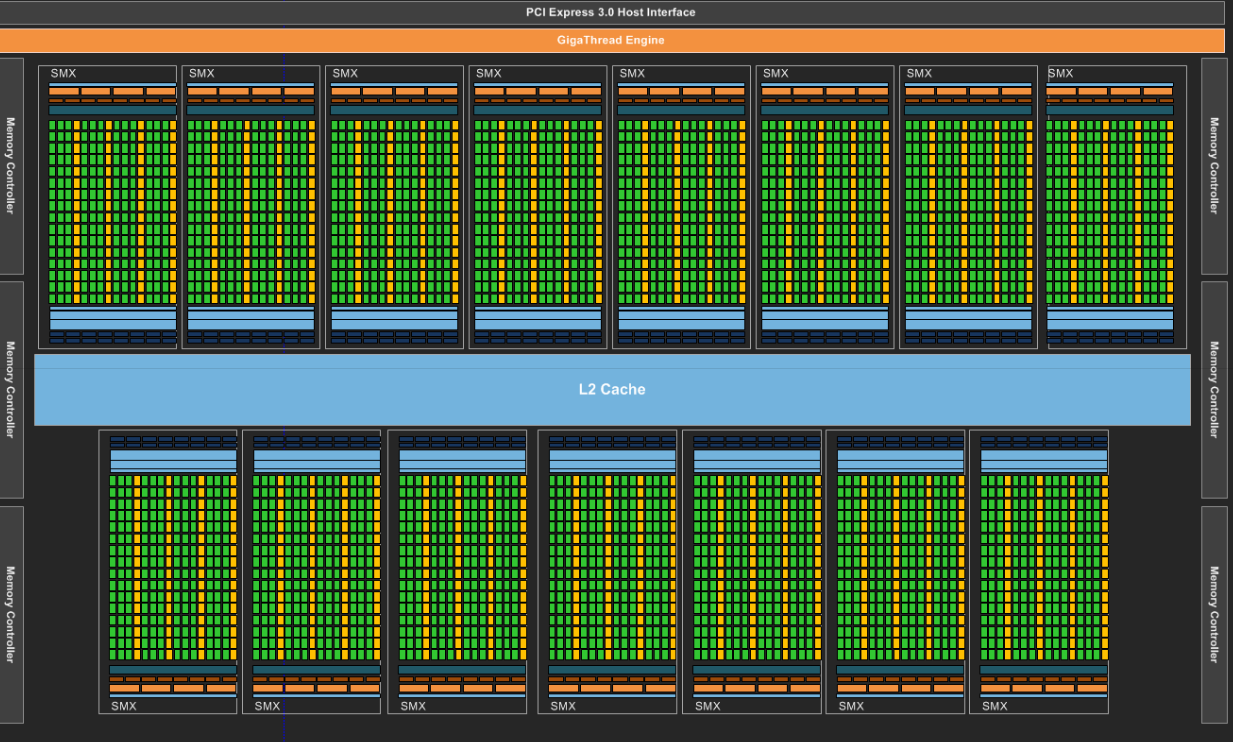
\includegraphics[width=1.0\textwidth]{kepler_1}
    \caption{Compute Units en Nvidia Kepler}
    \label{fig:kepler1}
\end{figure}

\begin{figure}[h]
    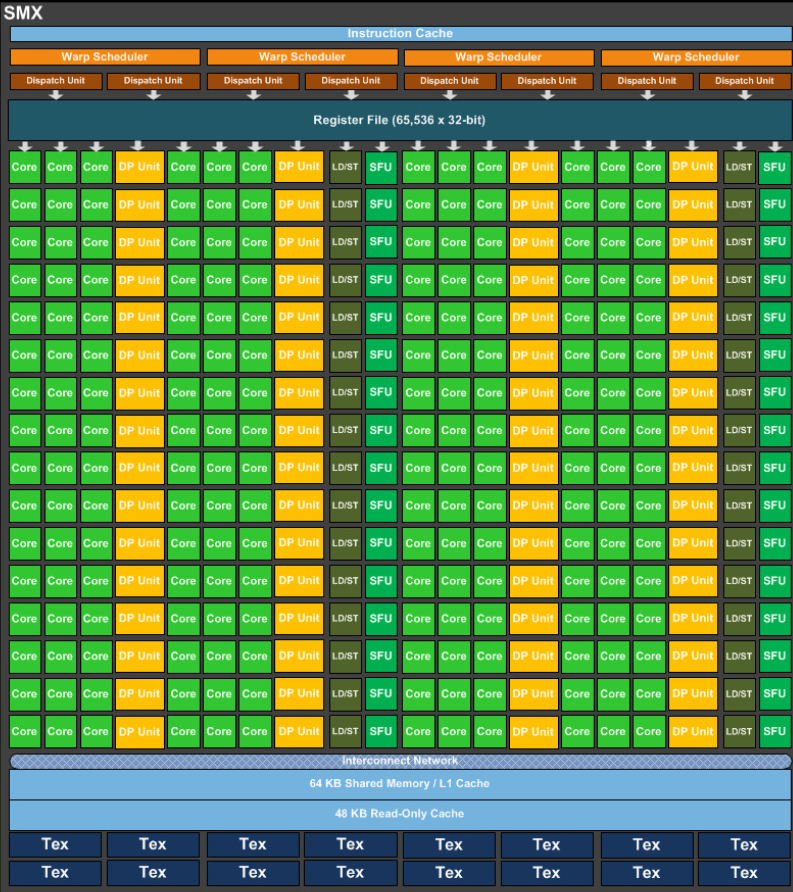
\includegraphics[width=1.0\textwidth]{kepler_2}
    \caption{Processing Elements Dentro de un Compute Unit}
    \label{fig:kepler2}
\end{figure}

\begin{figure}[ht]
    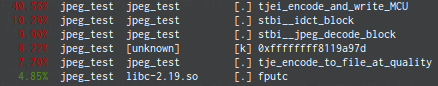
\includegraphics[width=4.5625in]{fputc}
    \caption{TinyJPEG: 48\%. fputc: 4.8\%}
\end{figure}

El kernel para nuestra función de selección va a hacer el trabajo de la función
\verb+encode_MCU+, que se encarga de tomar bloques de $8\times8$, codificarlos
y reportar el tamaño, y luego decodificarlos y reportar el error.

El kernel de DummyJPEG está diseñado para que cada \emph{work item} se encargue de un
bloque. Esto quiere decir que cada \emph{work item} puede estar procesando bloques
completamente distintos. Esto se hace porque cada bloque puede tener un número
arbitrario de ceros una vez que se ha aplicado la \gls{DCT} y se ha aplicado la
cuantificación. Si organizáramos el trabajo de manera que cada workgroup trabaje
con un solo bloque, cada \emph{wavefront} pasaría la mayor parte del tiempo esperando saltos
condicionales. El problema de los saltos condicionales se discute más adelante
en la sección \ref{sec:microopt}.

\begin {figure}
    \begin{tabular}{ | l | r | }
    \hline
    OpenCL             & Nvidia y CUDA \\
    \hline
    Work Item          & Thread \\
    Work Group         & Thread block \\
    Processing Element & CUDA Core \\
    Compute Unit       & Streaming Multiprocessor (SMX) \\
    \hline
    \end{tabular}
    \caption{Equivalencias Entre Términos usados en OpenCL y CUDA}
    \label{table:equiv}
\end{figure}

\section{Implementación paralela en CPU}

Para describir la versión paralela de \verb+encode_MCU+, primero hay que listar
los parámetros que toma la función secuencial, que es llamada una vez por cada
bloque.

\begin{enumerate}
    \item \verb+mcu+, el \emph{minimum coded unit}. Es decir, el bloque
        $8\times8$
    \item \verb+qt+, la tabla de cuantificación (puede ser de luminancia o
        crominancia)
    \item \verb+huffman+, apuntadores a las tablas de huffman para coeficientes
        DC y AC.
\end{enumerate}

Para todos los bloques, los elementos 2 y 3 se mantienen invariantes. Lo que se
hace es cambiar la función para que opere sobre un arreglo de bloques de
entrada y que escriba a un arreglo de salida.

Si hay $n$ bloques en la imagen, DummyJPEG procesa $n$ bloques a la vez y
escribe a un arreglo de $n$ resultados. Un resultado es una tupla $(b, e)$
donde $b$ es el número de bits que el bloque consume después de ser codificado
y $e$ es la suma de las diferencias absolutas pixel-por-pixel entre el bloque
original y el bloque descomprimido.

Como se quiere que la implementación paralela en el CPU sea tan similar al
kernel OpenCL final como sea posible, agregamos un nuevo parametro,
\verb+block_i+. Como su nombre sugiere, es un índice que indica el bloque al
que la función tiene que acceder y el índice a donde tiene que escribir su
resultado.

El algoritmo paralelo trabaja en un patrón \emph{map-reduce}. No en el sentido
de utilizar un cluster de computadoras para cómputo paralelo, si no en los
conceptos de programación funcional que motivaron el título. Es un algoritmo
estilo \emph{map-reduce} porque la mayor parte del cómputo se realiza en
paralelo sobre elementos de un arreglo (correspondiente a la función map) y
cuando el proceso paralelo termina, se realiza una recolección secuencial para
obtener  el resultado final (el equivalente a la función \emph{reduce}). Al implementar una
versión paralela de \verb+encode_MCU+, ya se tiene la función map. Entonces la
función \emph{reduce} consiste de:

\label{alg:mcu_paralelo}
\begin{code}
    B_total = 0;
    E_total = 0;
    Para todo resultado (B, E):
       B_total += B;
       E_total += E;
    Terminar el algoritmo, regresando (B_total, E_total).
\end{code}

La tupla que regresa DummyJPEG son los parámetros $e(T)$ y $s(T)$ de la función de selección
\ref{eq:fitness}.

En el cpu, la parte \emph{map} del algoritmo se ve así:

\begin{code}[language=C][h]
    // Versión de un solo hilo.
    for (int i = 0; i < num_bloques; ++i) {
        encode_MCU(i, mcus, qt, huffman);
    }
\end{code}

Para multihilo, se utilizan hilos de ejeuciones trabajadores que consumen unidades
de trabajo. Como se muestra con el siguiente pseudo código:

\begin{code}[language=C][h]
    bool loop = true;
    while ( loop ) {
        // Pseudo-código para el hilo trabajador

        int block_i = -1;

        // Sección crítica
        lock();
        if ( bloques_consumidos < num_bloques ) {
            int block_i = bloques_consumidos++;
        } else {
            loop = false;
        }
        unlock();

        if ( block_i >= 0 ) {
            encode_MCU(block_i, mcus, qt, huffman);
        }
    }
\end{code}

El producir trabajo se reduce a esto:

\begin{code}[language=C][h]
    // Apuntar al lugar correcto una variable que los
    // trabajadores puedan accesar.
    g_MCUs = mcus;

    // Cada trabajador lo incrementa atómicamente.
    bloques_consumidos = 0;

    lanzar_trabajadores();
\end{code}

\section{Paralelización en GPU}

Una vez que la implementación paralela funciona en el CPU, es hora de hacer la
implementación OpenCL de DummyJPEG. Como OpenCL usa un dialecto de C, se puede
reutilizar código entre las dos implementaciones de DummyJPEG. Se usa el mismo
código para la DCT y la IDCT. El kernel no es exactamente un \emph{copy paste},
pero la implementación es bastante parecida. Los únicos cambios que se realizan
son en la firma de la función, que tiene sintaxis de OpenCL para especificar
que la función es un kernel y para definir si los parámetros están en memoria
global o en memoria constante.

En la sección \ref{sec:gpgpu} no se habló de memoria constante porque es
operacionalmente igual a la memoria global. La ventaja de usar memoria
constante es que es más fácil de optimizar para el driver, por la garantía de no-escritura.

La firma del kernel \verb+encode_MCU+ es:

\begin{code}[language=C][h]
__kernel void
cl_encode_and_write_MCU(
    /*0*/__global DJEBlock* mcu_array,
    /*1*/__global uint* bitcount_array,
    /*2*/__global ulong* out_mse,
    /*3*/__global float* qt,
    /*4*/__constant uchar* huff_ac_len)
\end{code}

Como se discutió, se convierte \verb+encode_MCU+ en un kernel y se utiliza una
variable global de OpenCL para determinar el bloque con el que se está
trabajando.

\begin{code}[language=C][h]
    // Obtener el indice de bloque en OpenCL
    int block_i = (int)get_global_id(0);
\end{code}
{
La gran mayoría del esfuerzo en implementar la versión paralela en GPU es en
hacer la inicialización necesaria para que OpenCL establezca una línea de
comunicación entre el CPU y el GPU. Para referencia, ver los archivos
\verb+gpu.c+ y \verb+gpu.h+ en el código fuente del proyecto. Entre las cosas
que se necesitan hacer están: Encontrar un dispositivo OpenCL (el GPU,
idealmente, aunque OpenCL está diseñado para ser una API genérica); Crear un
contexto OpenCL, la estructura que mantiene el estado de la API; Y finalmente
compilar el kernel.

Durante la ejecución, se debe hacer el manejo de memoria de GPU. Todos los
parámetros del kernel son apuntadores a localidades de memoria global en el GPU
que se crean con OpenCL como objetos llamados \emph{OpenCL buffers}. Algunos de
ellos, como las tablas de Huffman, no cambian durante el programa. Otros, como
la tabla de cuantificación, cambia con cada llamada al kernel. Se tiene que
asegurar no tener \emph{memory leaks} y de no borrar buffers mientras están
siendo usados.

Aunque no es una API ideal, el trabajo de inicialización y de manejo de memoria
es relativamente fácil si uno sigue al pie de la letra la especificación de
OpenCL 1.1 \cite{opencl-spec}

Afortunadamente, la estrategia de hacer la implementación paralela en el CPU,
pensando en GPU, para después migrar el trabajo al GPU fue exitosa. La
implementación paralela en GPU requirió de sólo el mínimo esfuerzo necesario,
dejando tiempo para hacer las micro-optimizaciones que se describen en la
sección \ref{sec:microopt}.

El algoritmo funciona correctamente en tres modalidades: Un hilo, multihilo, y GPU. Para un conjunto de imágenes de prueba, la tabla
\ref{table:perf_table_orig} muestra el tiempo en segundos que cada modalidad toma
para realizar la evolución de la tabla de cuantificación y escribir el JPEG
resultante.

\begin{figure}[h]
    \begin{tabular}{ |l c c c c r| }
        \hline
        Nombre &  Un Hilo & Multihilo & GPU & Speedup MT & Speedup GPU \\
        \hline
        Diego & 10.796s & 5.210s & 1.391s  & 2.072X & 7.76X \\
        Ghost & 13.706s & 6.607s & 1.760s  & 2.257X & 7.78X \\
        Klay & 40.526s & 22.279s & 4.785s  & 1.819X & 8.46X \\%, 4.65
        Plutón & 558.83s & 204.120s & 13.940s & 2.73X & 40.08X \\ % 14.64
        \hline
    \end{tabular}
    \caption{Tabla de desempeño para gp\_encoder}
    \label{table:perf_table_orig}
\end{figure}

Más adelante se describen las características de las cuatro imágenes de prueba
\ref{sec:testset}. Cabe notar que aunque la implementación GPU es siempre más
rápida, en el caso de la imagen ``Plutón", que mide 192MB, el beneficio del GPU
crece por un factor de alrededor de 5X comparándolo con la modalidad CPU con un
hilo. Es posible que la razón sea que el trabajo a realizar crece
proporcionalmente con el tamaño de la imagen, y los GPU están diseñados para
rendimiento, no latencia. Se puede especular sobre la razón verdadera. Puede
que el hecho de que haya más wavefronts en vuelo permita que los \emph{ Compute Units }
tengan una mayor utilización, mientras que el menor número de wavefronts para
las imágenes más pequeñas cause problemas de utilización cuando muchos
\emph{wavefront}s están ejecutando código con saltos condicionales, como el proceso en
JPEG en el que se busca el útlimo elemento del bloque que no es cero. Otra
explicación sería que con imágenes grandes, el calendarizador puede hacer un
mejor trabajo dándole la vuelta a problemas de contención de memoria.


% ============================================================
\section{Algoritmo DCT} \label{sec:DCT}
% ============================================================

A partir de la ecuacion \ref{eq:dct} se puede derivar directamente un algoritmo
simple para la \emph{DCT}:

\begin{figure}
    \begin{code}[language=C][h]
        float DCT[64];
        for (int v = 0; v < 8; ++v) {
            for (int u = 0; u < 8; ++u) {
                DCT[v*8 + u] = F(u, v);
                // F es la traducción directa de definición DCT
            }
        }
    \end{code}
    \caption{Algoritmo DCT derivado directamente}
    \label{alg:dct}
\end{figure}

\verb+tiny_jpeg+ contiene dos implementaciones de \emph{DCT}, la que se deriva
directamente de la ecuación \ref{eq:dct} y que muestra en la tabla \ref{alg:dct}.

El algoritmo \ref{alg:dct} no es práctico para un codificador JPEG y mucho
menos para este proyecto, que ejecuta el algoritmo JPEG cientos de veces para
una sola imagen. Existen métodos para calcular la DCT (y su inversa, la IDCT)
rápidamente. La discusión presentada aquí sobre el desarrollo de algoritmos
rápidos DCT es análoga para la inversa, ya que las ecuaciones son muy similares
(\ref{eq:dct}, \ref{eq:idct}).

Este proyecto usa el algoritmo \gls{DCT} usado en proyectos como ffmpeg y la
implementación de referencia de JPEG. Fue originalmente desarrollado por
\cite{ahmed_dct}.

El algoritmo está basado en la observación de que la ecuación \ref{eq:dct} es
lineal, y por lo tanto el cálculo \emph{DCT} se puede expresar como $F(X) =
A^{T}XA$ Donde $X$ es un bloque de $8\times8$ y A es la matriz:

\begin{equation}
    \label{eq:dct-matrix}
    \begin{bmatrix}
        \frac{\sqrt{2}}{2} & \frac{\sqrt{2}}{2} & \frac{\sqrt{2}}{2} & \frac{\sqrt{2}}{2} & \frac{\sqrt{2}}{2} & \frac{\sqrt{2}}{2} & \frac{\sqrt{2}}{2} & \frac{\sqrt{2}}{2} \\
        cos\frac{\pi}{16} & cos\frac{3\pi}{16}& cos\frac{5\pi}{16}& cos\frac{7\pi}{16}& cos\frac{9\pi}{16}& cos\frac{11\pi}{16}& cos\frac{13\pi}{16}& cos\frac{15\pi}{16} \\
        cos\frac{2\pi}{16} & cos\frac{6\pi}{16}& cos\frac{10\pi}{16}& cos\frac{14\pi}{16}& cos\frac{18\pi}{16}& cos\frac{22\pi}{16}& cos\frac{26\pi}{16}& cos\frac{30\pi}{16} \\
        cos\frac{3\pi}{16} & cos\frac{9\pi}{16}& cos\frac{15\pi}{16}& cos\frac{21\pi}{16}& cos\frac{27\pi}{16}& cos\frac{33\pi}{16}& cos\frac{39\pi}{16}& cos\frac{45\pi}{16} \\
        cos\frac{4\pi}{16} & cos\frac{12\pi}{16}& cos\frac{20\pi}{16}& cos\frac{28\pi}{16}& cos\frac{36\pi}{16}& cos\frac{44\pi}{16}& cos\frac{52\pi}{16}& cos\frac{60\pi}{16} \\
        cos\frac{5\pi}{16} & cos\frac{15\pi}{16}& cos\frac{25\pi}{16}& cos\frac{35\pi}{16}& cos\frac{45\pi}{16}& cos\frac{55\pi}{16}& cos\frac{65\pi}{16}& cos\frac{75\pi}{16} \\
        cos\frac{6\pi}{16} & cos\frac{18\pi}{16}& cos\frac{30\pi}{16}& cos\frac{42\pi}{16}& cos\frac{54\pi}{16}& cos\frac{66\pi}{16}& cos\frac{78\pi}{16}& cos\frac{90\pi}{16} \\
        cos\frac{7\pi}{16} & cos\frac{21\pi}{16}& cos\frac{35\pi}{16}& cos\frac{49\pi}{16}& cos\frac{63\pi}{16}& cos\frac{77\pi}{16}& cos\frac{91\pi}{16}& cos\frac{105\pi}{16}
    \end{bmatrix}
\end{equation}

Esta matriz tiene alta redundancia. Por ejemplo, el cuarto elemento del segundo renglón es $cos\frac{7\pi}{16} \approx 0.19509$. Este va a ser el mismo valor para todos los elementos que sean $cos\frac{n\pi}{16}$ con $n \mod 16 = 7$. Dígase $\frac{25\pi}{16}$, y $\frac{39\pi}{16}$.

Para simplificar la representación se usa el módulo 16 como se acaba de mostrar junto con dos técnicas más: la periodicidad del coseno: $\Big( cos(x) = cos(x + 2\pi) \Big)$ y la propiedad de que es una función par: $\Big( cos(-x) = -cos(x) \Big)$.

Se termina con una matriz cuyos elementos tienen 7 posibles valores y sus negativos:

\begin{equation}
    \label{eq:dct-matrix-simple}
    \sqrt{2}/2
    \begin{bmatrix}
        1 & 1 & 1 & 1 & 1 & 1 & 1 & 1  \\
        a & c & d & f & -f & -d & -c & -a \\
        b & e & -e & -b & -b & -e & e & b \\
        c & -f & -a & -d & d & a & f & -c \\
        1 & -1 & -1 & 1 & 1 & -1 & -1 & 1\\
        d & -a & f & c & -c & -f & a & -d \\
        e & -b & b & -e & -e & b & -b & e \\
        f & -d & c & -a & a & -c & d & -f
    \end{bmatrix}
\end{equation}

donde

\begin{eqnarray*}
    a = \frac{2}{\sqrt{2}}cos\frac{\pi}{16}\\
    b = \frac{2}{\sqrt{2}}cos\frac{\pi}{8}\\
    c = \frac{2}{\sqrt{2}}cos\frac{3\pi}{16}\\
    d = \frac{2}{\sqrt{2}}cos\frac{5\pi}{16}\\
    e = \frac{2}{\sqrt{2}}cos\frac{3\pi}{8}\\
    f = \frac{2}{\sqrt{2}}cos\frac{7\pi}{16}
\end{eqnarray*}

Si aplicamos la ecuación $F(X) = A^{T}XA$ se va a observar que toda columna de la matriz $Y = F(X)$ se ve así:

\begin{equation}
    \label{eq:dct-row}
    \begin{bmatrix}
        Y_0 \\
        Y_2 \\
        Y_4 \\
        Y_6
    \end{bmatrix}
    = \frac{\sqrt{2}}{2} \begin{bmatrix}
        1 & 1 & 1 & 1  \\
        b & e & -e & -b \\
        1 & -1 & -1 & 1  \\
        e & -b & b & e
        \end {bmatrix} \begin {bmatrix}
        X_0 + X_7 \\
        X_1 + X_6 \\
        X_2 + X_5 \\
        X_3 + X_4
        \end {bmatrix}
\end{equation}

\begin{equation*}
    \begin{bmatrix}
        Y_1 \\
        Y_3 \\
        Y_5 \\
        Y_7
    \end{bmatrix}
    = \frac{\sqrt{2}}{2} \begin{bmatrix}
        a & -c & d & -f  \\
        c & f & -a & d  \\
        d & a & f & -c  \\
        f & d & c & a
        \end {bmatrix} \begin {bmatrix}
        X_0 - X_7 \\
        X_6 - X_1 \\
        X_2 - X_5 \\
        X_4 - X_3
        \end {bmatrix}
\end{equation*}

donde $X$ es un renglón del bloque original.

De esta ecuación sacamos directamente el algoritmo final. Avanzamos por las 8 columnas del bloque original, escribiendo a los 8 renglones del bloque DCT.

Para ilustrar la diferencia entre el algoritmo directo y el algoritmo que se describe aquí, se incluyen dos imágenes de una aplicación que carga una imagen de prueba y la codifica con TinyJPEG. Se deshabilita la optimización para que no se hagan optimizaciones \emph{inline}, pero los resultados son consistentes con niveles altos de optimización.

Nótese que la figura \ref{fig:pre_dct} muestra al algoritmo DCT tomando un total de 98.76\% del tiempo total del programa, mientras que en la figura \ref{fig:post_dct} está reducido a un 12.34\%.

\begin{figure}[h]
    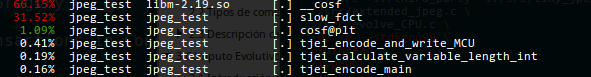
\includegraphics[width=1.0\textwidth]{pre_dct}
    \caption{Algoritmo DCT lento}
    \label{fig:pre_dct}
\end{figure}

\begin{figure}[h]
    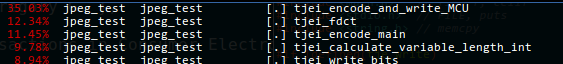
\includegraphics[width=1.0\textwidth]{post_dct}
    \caption{Algoritmo DCT rápido}
    \label{fig:post_dct}
\end{figure}


% ============================================================
\section{Micro-Optimización} \label{sec:microopt}
% ============================================================


Usamos el término \emph{micro-optimización} cuando nos referimos al tipo de
optimización de desempeño en la que no cambiamos los algoritmos que utilizamos.
Utilizamos conocimiento sobre la máquina o máquinas que van a
efectuar el cómputo para hacer cambios en la manera en que se ejecuta nuestro
algoritmo con el objetivo de obtener un mejor desempeño.

Un ejemplo de optimización que \emph{no} es micro-optimización es la
descripción del algoritmo DCT mostrado en \ref{sec:DCT}. En este ejemplo, se
logró tomar el cuello de botella de la implementación JPEG y reducirla a algo
mucho menos significativo mediante cambios algorítmicos.

Hacer micro-optimización no es recomendable hasta que uno esté seguro de que no
hay mejoras algorítmicas que puedan beneficiar el desempeño. La
micro-optimización casi siempre resulta en más código que es más difícil de
mantener. Sin embargo, cuando se llega al punto en donde no hay (o no se
ocurren) mejoras algorítmicas, podemos acelerar significativamente nuestro
programa con micro-optimización.

\subsection{GPU: Copiar bloques}

En la microarquitectura de un GPU, accesos a la memoria global usualmente
resultan en que la memoria sea copiada automáticamente a memoria local, de la
misma manera que se utilizan cachés en CPU para lidiar con la latencia de la
memoria principal. Sin embargo, no siempre podemos contar con que esto va a
suceder.

Cuando se sabe que un \emph{work item} va a trabajar con un trozo de memoria de cierto
tamaño, ocasionalmente es buena idea forzar una copia a memoria local para
reducir el tiempo que el \emph{work item} está esperando a memoria principal. El
siguiente pseudocódigo es una optimización común en OpenCL.

\label{alg:gpgpu-memcpy}
\begin{code}[language=C][h]
    // 64 es un número arbitrario.
    // Hay que tomar en cuenta el tamaño de la memoria local.
    int mi_copia[64];
    for (int i = 0; i < 64; ++i) {
        mi_copia[i] = memoria_global[i];
    }
\end{code}

En el caso de nuestro kernel, esta optimización resulta efectiva cuando
copiamos el \gls{MCU} (512 bytes). En la tabla \ref{table:gpucopy} se compara el tiempo
total de nuestro programa, con tres imágenes de prueba, haciendo una copia
local vs memoria global.

\begin{figure}[h]
    \begin{tabular}{ |l c c r| }
        \hline
        Imagen & Memoria local & Memoria global & \emph{speedup} \\
        \hline
        Klay & 3.85 & 4.5 & 1.168 \\
        Diego & 1.18 & 1.44 & 1.22 \\
        Plutón & 40.16 & 47.58 & 1.1847 \\
        \hline
    \end{tabular}
    \caption{Comparación de desempeño para copia local de bloques}
    \label{table:gpucopy}
\end{figure}

Logramos una mejora de entre 16\% y 22\% haciendo lo que a primera vista parece
más trabajo. Cabe notar que no se logra la misma mejora copiando otros
parámetros de entrada, como las tablas Huffman. Es posible que se obtiene este
desempeño adicional porque se está cargando a memoria local \emph{toda} la
memoria del bloque que va a accesarse por ese \emph{work item}, mientras que el acceso
a las tablas de Huffman es mucho más aleatorio y son arreglos mucho más
grandes.

\subsection{GPU: Saltos condicionales}

Un \emph{ salto condicional } es en lo que se convierte un \verb+if+ cuando
se compila a código máquina. Para observar por qué los saltos condicionales
(usualmente llamados \emph{branches} para ahorrar teclas) son un problema en
GPU, vale la pena hacer un ejemplo.

Supóngase que un \emph{wavefront} ejecuta el siguiente código:

\begin{code}[language=C][h]
    if (mi_variable) {
        funcion_a();
    } else {
        funcion_b();
    }
    funcion_c();
\end{code}

También supóngase que \verb+mi_variable+ es \verb+true+ para el 90\% de los work
items.  Cuando se llega al \verb+if+, 90\% de los \emph{work items} van a ejecutar
\verb+funcion_a+, mientras que el 10\% restante va a ejecutar \verb+funcion_b+.
El problema está en que no se puede ejecutar \verb+funcion_c+ hasta que todos
los \emph{work items} en el \emph{wavefront} hayan terminado de ejecutar el bloque if. Esto
quiere decir que si \verb+funcion_b+ es muy cara, el 90\% del \emph{wavefront} va a
estar sin hacer trabajo, esperando a que el 10\% restante termine de ejecutar
\verb+function_b+.

El kernel de DummyJPEG no puede hacer mucho para evitar que haya \emph{wavefront}s
esperando saltos condicionales. Esto es por la naturaleza del algoritmo JPEG.
El procesamiento de un bloque requiere contar el número de coeficientes que son
cero, y para hacer esto es necesario iterar por todo el bloque. Encima de esto,
cada bloque tiene una cantidad de trabajo proporcional al número de
aoeficientes que no son cero. Esto implica que cualquier \emph{wavefront} de DummyJPEG
va a esperar al \emph{work item} que tenga el menor número de ceros que procesar y por
lo tanto más trabajo que hacer.

Estar conscientes de que la palabra \verb+if+ puede ser la parte más costosa
del programa es una de las diferencias más claras cuando se hace programación
\gls{GPGPU}.


\subsection{CPU: I/O} \label{sub:cpu-io}

TinyJPEG mantiene un \emph{buffer} de 1024 bytes que se usa para minimizar
llamadas a fwrite. Las implementaciones de fwrite tratan de evitar llamadas a
sistema, pero de cualquier manera, el uso de este buffer reduce dramáticamente
el costo de escritura.

La figura \ref{fig:fwrite} muestra el costo de fwrite en TinyJPEG con buffering
deshabilitado.

\begin{figure}[hb]
    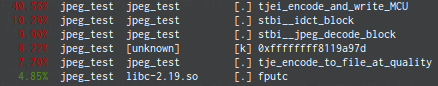
\includegraphics[width=5.16666in]{fputc}
    \caption{El costo de fwrite sin buffering}
    \label{fig:fwrite}
\end{figure}

Este reporte de la herramienta \verb+perf+, parte de Linux Perf Tools
\cite{linux-perf-tools}, es de un programa de prueba que carga una imagen de
Plutón de 192 MB y la codifica con TinyJPEG. Lo que se muestra es que hay dos
funciones de TinyJPEG consumiendo el 48.2\% del tiempo. También muestra que la
función \verb+fputc+ consume 4.8\% del tiempo total. Con esto concluímos que si
solo tomamos en cuenta el tiempo que se pasa codificando la imagen, se está
gastando el 9.1\% del tiempo llamando a fwrite, (que a su vez llama a putc).

No se incluye un reporte de TinyJPEG con \emph{buffering} porque al usar un
buffer de 1024 bytes, eliminamos por completo el costo de \verb+fwrite+.

La implementación de un buffer es muy simple. Este código viene directamente de TinyJPEG:

\begin{code}[language=C][h]
    // Buffer TJE_BUFFER_SIZE in memory and flush when ready
    static size_t tjei_g_output_buffer_count;
    static uint8_t tjei_g_output_buffer[TJEI_BUFFER_SIZE];
\end{code}

La manera en que nos deshacemos del problema de fwrite es escribiendo a ese
buffer.  Cuando tjei\_g\_output\_buffer\_count es igual a TJEI\_BUFFER\_SIZE,
entonces llamamos fwrite, escribiendo los contenidos del buffer completo.

Vale la pena notar que al final de la ejecución es probable que haya datos en
el buffer que no hayan sido escritos. Por eso se hace un \emph{flush} al final
del programa, haciendo una última llamada a fwrite con los contenidos del
buffer.

\subsection{CPU: Saltos condicionales}\label{sub:cpu-branch}

Para terminar las notas de micro-optimización, se va a discutir un truco en la
implementación de TinyJPEG que trata con predicción de \emph{branches} (i.e.
saltos condicionales, o bloques \verb+if+)

Los CPU son muy buenos ejecutando \emph{branches} cuando pueden predecir su
comportamiento. Agner Fog \cite{agner} tiene muy buenos recursos para estar al
día con la manera en que los procesadores de Intel predicen branches. El
concepto es que cuando el CPU piensa que un branch va a ser ejecutado, lo
ejecuta \emph{ especulativamente } mientras la condición del salto se computa
paralelamente. Se le conoce como un \emph{branch missprediction}, que
traducimos como \emph{mis-predicción de salto} a la situación en cuando el
salto se calculó especulativamente pero la condición falló. En código de alto
desempeño como la función interna de JPEG, esto puede ser un cuello de botella.

En el caso e TinyJPEG, una vez que se utilizó un algoritmo rápido de DCT, el
cuello de botella en la función \verb+encode_MCU+ resultó ser la siguiente
línea de código:

\begin{code}[language=C][h]
fval = (fval > 0)? floorf(fval + 0.5f) : ceilf(fval - 0.5f);
\end{code}

Esta es una implementación clásica de redondeo, escrita de acuerdo a la
especificación JPEG.

Usando \verb+perf+, se puede visualizar el problema (figura \ref{fig:mispred}):

\begin{figure}[h]
    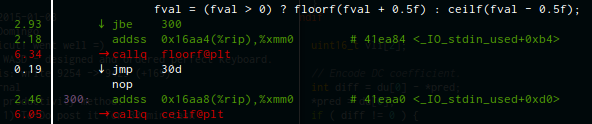
\includegraphics[width=5.16666in]{round_slow}
    \caption{Mis-predicción de salto}
    \label {fig:mispred}
\end{figure}

Ambos caminos del salto condicional inducido por el operador \verb+?:+ toman
alrededor de 9\% de los ciclos de CPU totales para esta función, con un total de 18\%.

Esa información no es suficiente para decidir que el problema es
mis-predicción, pero se puede atacar al problema como si fuera un problema de
mis-predicción. Si se hace más rápido, entonces suponemos que el problema era
el salto.

En este caso, sabemos que $fval \in [-1024, 1024]$. Esta información nos
permite evitar el salto haciendo una suma, $(fval + 1024) \in [0, 2048]$. Si
hacemos esto, podemos usar \verb+floorf+, ya que el valor siempre es positivo:

\begin{code}[language=C][h]
    fval += 1024;
    fval = floorf(fval + 0.5f);
    fval -= 1024;
\end{code}

El resultado, con \verb+perf+:

\begin{figure}[hb]
    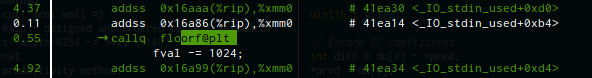
\includegraphics[width=5.16666in]{round_fast}
    \caption{Evitando mis-predicción}
\end{figure}

Como logramos alrededor de 2X de mejora en velocidad, podemos concluir con
confianza que el salto no se estaba prediciendo exitosamente, con el resultado
de que \verb+floorf+ y \verb+ceilf+ se estaban calculando \emph{siempre},
independientemente de si \verb+fval+ era positivo o negativo.



